\documentclass[tikz,border=10pt]{standalone}
\usepackage{tikz}
\usetikzlibrary{positioning}

\begin{document}

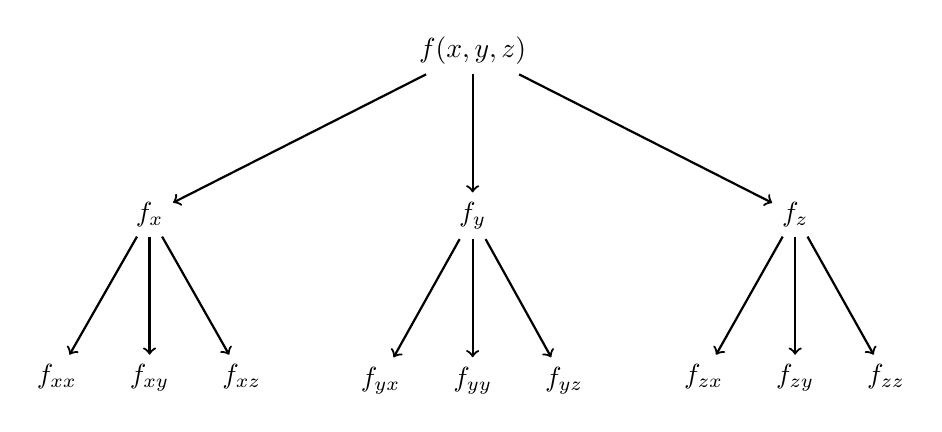
\begin{tikzpicture}[node distance=15mm and 30 mm, arrow/.style={->, thick}, scale = 2] %u node distance prvo ide vertikalni, a onda horizontalni razmak

%prva razina slike
\node (f) {$f(x,y,z)$};

%druga razina slika
\node (fx) [below left=of f] {$f_x$};
\node(fy)[below = of f]{$f_y$};
\node (fz)[below right=of f]{$f_z$};

%treća razina slike
\begin{scope}[node distance=15mm and 5mm]
    \node (fxx) [below left=of fx] {$f_{xx}$};
    \node (fxy) [below=of fx] {$f_{xy}$};
    \node(fxz)[below right = of fx]{$f_{xz}$};
    \node (fyx) [below left=of fy] {$f_{yx}$};
    \node (fyy) [below =of fy] {$f_{yy}$};
    \node(fyz)[below right = of fy]{$f_{yz}$};
    \node(fzx)[below left  = of fz]{$f_{zx}$};
    \node(fzy)[below = of fz]{$f_{zy}$};
    \node(fzz)[below right = of fz]{$f_{zz}$};
\end{scope}

%strelice od f prema parcijalnim derivacijama
\draw[arrow] (f) -- (fx);
\draw[arrow] (f) -- (fy);
\draw[arrow] (f)--(fz);

%strelice od parcijalnih derivacije prema derivacijama drugog reda
\draw[arrow] (fx) -- (fxx);
\draw[arrow] (fx) -- (fxy);
\draw[arrow] (fx) -- (fxz);
\draw[arrow] (fy) -- (fyx);
\draw[arrow] (fy) -- (fyy);
\draw[arrow] (fy) -- (fyz);
\draw[arrow] (fz) -- (fzx);
\draw[arrow] (fz) -- (fzy);
\draw[arrow] (fz) -- (fzz);

\end{tikzpicture}

\end{document}
